\documentclass[xcolor=table,handout]{beamer}
\setbeamertemplate{navigation symbols}{}

\usepackage{pgfpages}
\usepackage{adjustbox}
\setbeameroption{show notes}
\setbeameroption{show notes on second screen=right}

\usepackage{booktabs}
\usepackage{beamerthemeshadow}
\setbeamertemplate{caption}[numbered]
\setbeamerfont{caption}{size=\tiny}

\begin{document}

\title{Journal Club Presentation: Ocean Color}  
\author[K. Bellock, L. Chen, D. Durrance, A. Yen, H. Perez]{Kenneth Bellock, Leshi Chen, Danielle Durrance, Andrew Yen, Hack Perez}
\titlegraphic{%
    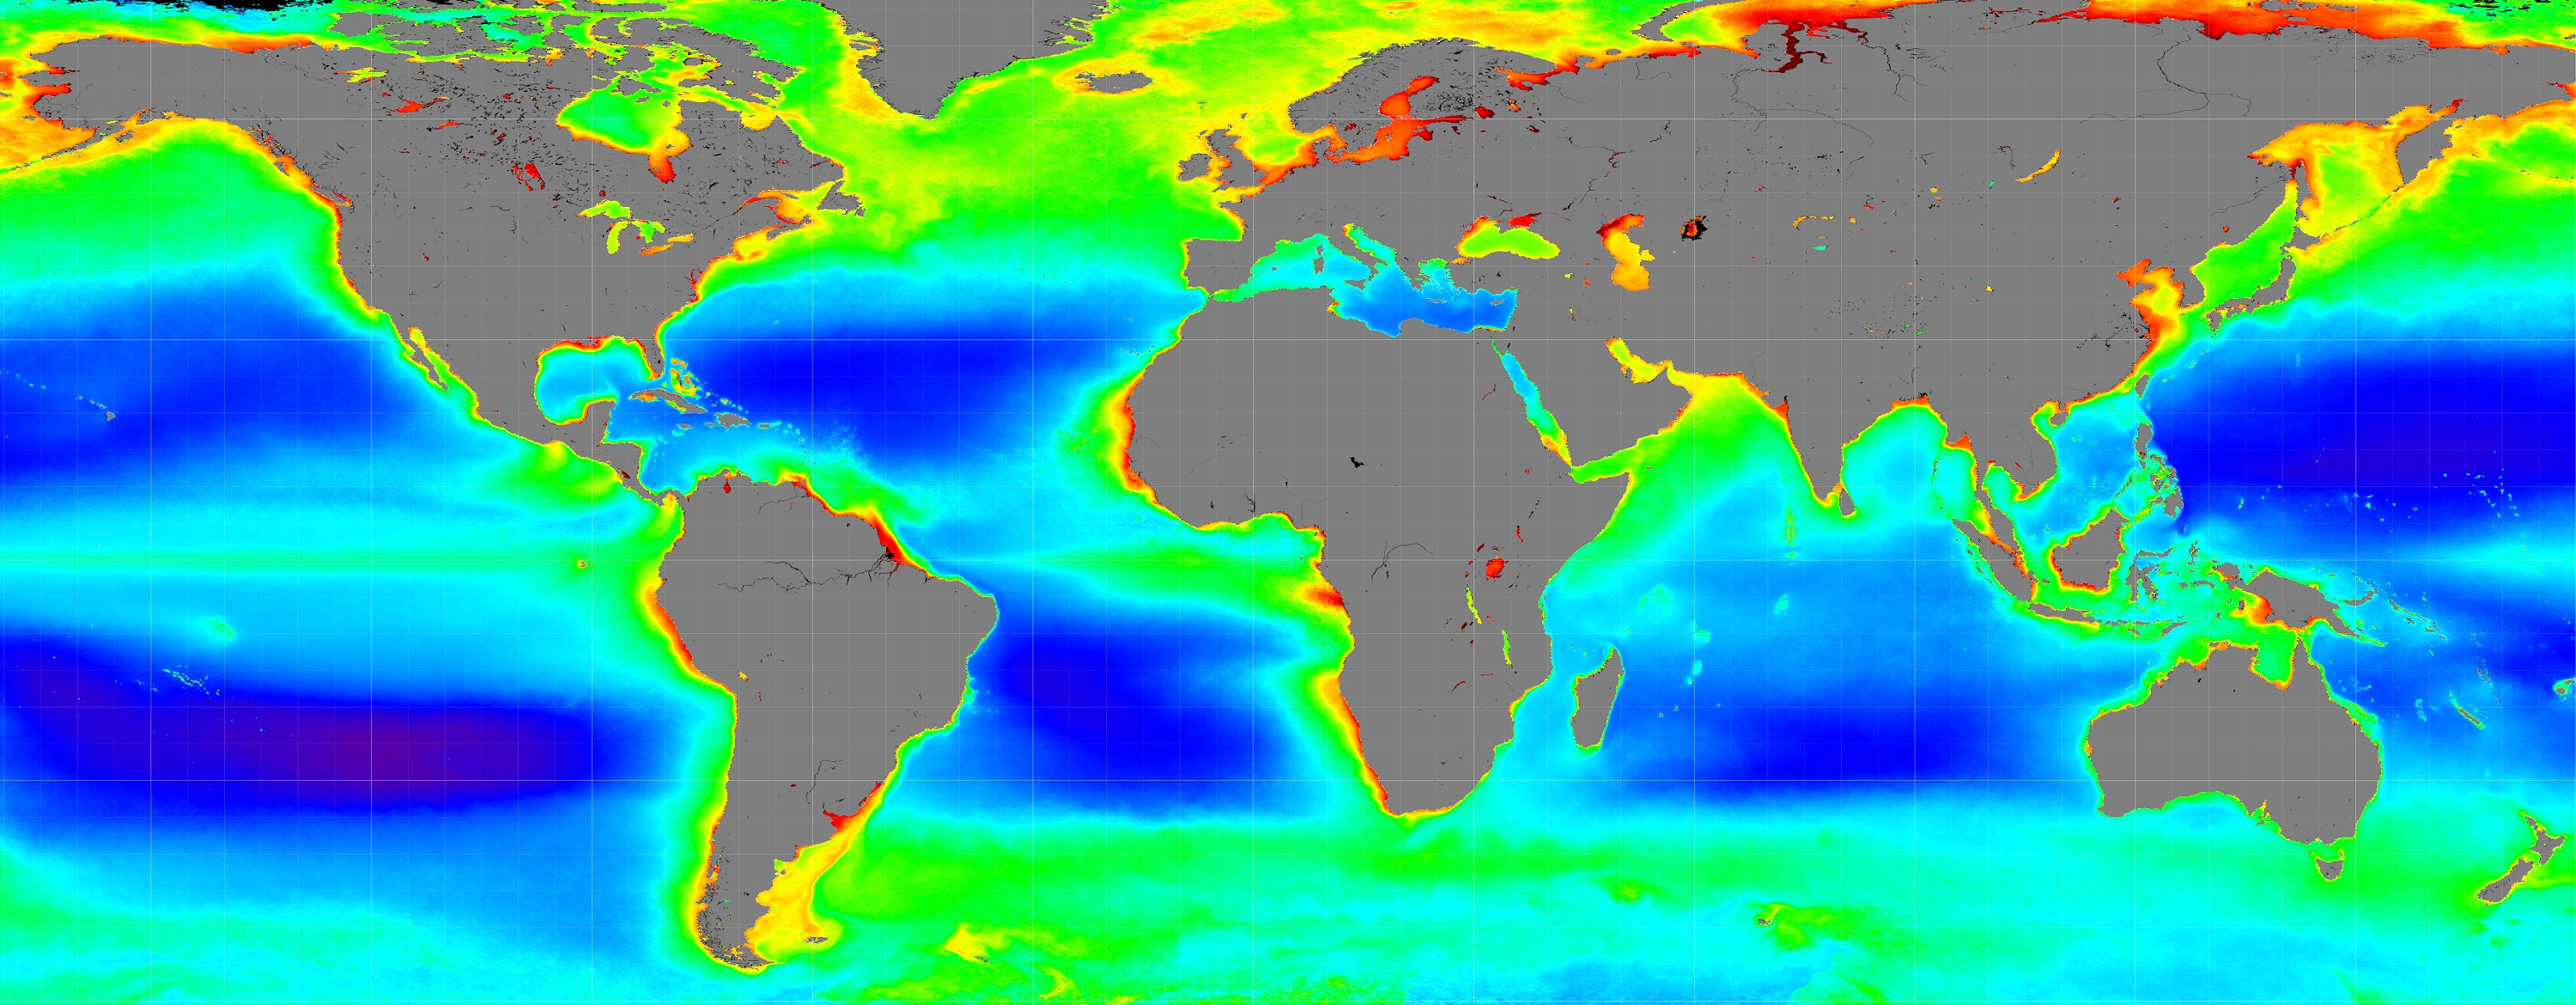
\includegraphics[height=.37\textheight]{15_037}

    \tiny \textbf{Source:} \url{https://www.nasa.gov/press/2015/march/new-nasa-mission-to-study-ocean-color-airborne-particles-and-clouds}
}
\date{\vspace*{-2.5em}\par April 4, 2018} 

\section{Introduction}

\begin{frame}
  \titlepage{}
  \note{Assumptions:}
  \note[item]{TODO:\@ List assumptions.}
\end{frame}

\begin{frame}\frametitle{Table of contents}
  \tableofcontents{}
  \note[item]{A road map is a great thing to have.}
  \note[item]{A joke or reference to current events in common culture would be great here if the audience appears receptive.}
\end{frame} 

\begin{frame}\frametitle{Introduction} 

  \note[item]{TODO:\@ Write Introduction}
\end{frame}


\section{Article Summaries}

\begin{frame}\frametitle{Paper 1} 

  \note[item]{TODO:\@ Include title, authors, objectives, methods, findings, and at least one informative image or graph.}
\end{frame}

\begin{frame}\frametitle{Paper 1 (Continued)} 

  \note[item]{TODO:\@ Include title, authors, objectives, methods, findings, and at least one informative image or graph.}
\end{frame}

\begin{frame}\frametitle{Paper 2} 

  \note[item]{TODO:\@ Include title, authors, objectives, methods, findings, and at least one informative image or graph.}
\end{frame}

\begin{frame}\frametitle{Paper 2 (Continued)} 

  \note[item]{TODO:\@ Include title, authors, objectives, methods, findings, and at least one informative image or graph.}
\end{frame}

\begin{frame}\frametitle{Paper 3} 

  \note[item]{TODO:\@ Include title, authors, objectives, methods, findings, and at least one informative image or graph.}
\end{frame}

\begin{frame}\frametitle{Paper 3 (Continued)} 

  \note[item]{TODO:\@ Include title, authors, objectives, methods, findings, and at least one informative image or graph.}
\end{frame}

\begin{frame}\frametitle{Paper 4} 

  \note[item]{TODO:\@ Include title, authors, objectives, methods, findings, and at least one informative image or graph.}
\end{frame}

\begin{frame}\frametitle{Paper 4 (Continued)} 

  \note[item]{TODO:\@ Include title, authors, objectives, methods, findings, and at least one informative image or graph.}
\end{frame}


\section{Summary and Conclusion}

\begin{frame}\frametitle{Summary} 

  \note[item]{TODO:\@ Write Summary}
\end{frame}

\begin{frame}\frametitle{Conclusion} 

  \note[item]{TODO:\@ Write Conclusion}
\end{frame}


\end{document}
